% ****** Start of file apssamp.tex ******
%
%   This file is part of the APS files in the REVTeX 4.1 distribution.
%   Version 4.1r of REVTeX, August 2010
%
%   Copyright (c) 2009, 2010 The American Physical Society.
%
%   See the REVTeX 4 README file for restrictions and more information.
%
% TeX'ing this file requires that you have AMS-LaTeX 2.0 installed
% as well as the rest of the prerequisites for REVTeX 4.1
%
% See the REVTeX 4 README file
% It also requires running BibTeX. The commands are as follows:
%
%  1)  latex apssamp.tex
%  2)  bibtex apssamp
%  3)  latex apssamp.tex
%  4)  latex apssamp.tex
%
\documentclass[%
 reprint,
%superscriptaddress,
%groupedaddress,
%unsortedaddress,
%runinaddress,
%frontmatterverbose, 
%preprint,
%showpacs,preprintnumbers,
%nofootinbib,
%nobibnotes,
%bibnotes,
 amsmath,amssymb,
 aps,
%pra,
%prb,
%rmp,
%prstab,
%prstper,
%floatfix,
]{revtex4-1}

\usepackage{graphicx}% Include figure files
\usepackage[utf8]{inputenc}
\usepackage{dcolumn}% Align table columns on decimal point
\usepackage{bm}% bold math
%\usepackage{hyperref}% add hypertext capabilities
%\usepackage[mathlines]{lineno}% Enable numbering of text and display math
%\linenumbers\relax % Commence numbering lines

%\usepackage[showframe,%Uncomment any one of the following lines to test 
%%scale=0.7, marginratio={1:1, 2:3}, ignoreall,% default settings
%%text={7in,10in},centering,
%%margin=1.5in,
%%total={6.5in,8.75in}, top=1.2in, left=0.9in, includefoot,
%%height=10in,a5paper,hmargin={3cm,0.8in},
%]{geometry}

\begin{document}

\preprint{APS/123-QED}

\title{Radiactividad}% Force line breaks with \\
\thanks{}%

\author{Jesus Prada}
 \email{jd.prada1760@uniandes.edu.co}
 \altaffiliation[Also at ]{Departamento de Física, Universidad de los Andes}%Lines break automatically or can be forced with \\
\author{Sergio Iv\'an Rey}%
 \email{si.rey1826@uniandes.edu.co}
\affiliation{%
 Departamento de Física, Universidad de los Andes
}%

\date{10/09/2015}% It is always \today, today,
             %  but any date may be explicitly specified

\begin{abstract}
Durante este laboratorio se pretendía estudiar los fenómenos ondulatorios de las microondas en distintas configuraciones. En primer lugar se verificó el ángulo de máxima reflexión de las microondas al hacerlas incidir sobre una película metálica. Se comprobó que el ángulo de mayor reflexión es el mismo ángulo que el ángulo incidente con una precisión de $\pm2^o$. Asimismo, durante varias prácticas se determinó experimentalmente la longitud de onda de las microondas. Esto se llevó a cabo usando, en primer lugar un montaje para simular ondas estacionarias con el receptor actuando como reflector parcial. En segunda instancia se midió la longitud de onda mirando el patrón de interferencia de una doble rendija. De la misma manera, se determinó esta longitud de onda usando los interferómetros de Fabry-Perot, Michelson y el espejo de Lloyd. Para todos los casos, se encontró una longitud de onda dentro de los límites esperados obteniendo así un valor con error mínimo dado por $\lambda = 2.86cm$ ($0.1\%$) y un error máximo dado por $\lambda= 2.22cm$ ($22\%$). Se midieron asimismo los fenómenos de polarización, haciendo uso de las cabezas movibles que disponía el equipo de microondas, en donde se encontró como era esperado, la relación de intensidad proporcional a la componente que se dejaba pasar. Similarmente, haciendo uso de partículas pequeñas de estireno ubicadas dentro de un prisma se comprobó el fenómeno de refracción y se comprobó la Ley de Snell, como también pudo encontrarse, con un valor del índice de refracción de $n = 1.41$ ($11\%$ de error) el cual es muy cercano al nominal. Finalmente, haciendo uso del estireno, se diseñó una manga llena de estas partículas que serviría como fibra óptica con la cual se comprobó que la onda se transmitía sin pérdida de energía por este elemento. \\
\end{abstract}


\keywords{Microondas, refracción, reflexión, interferencia, fibra óptica, espejo de Lloyd, interferómetro de Michelson, interómetro de Fabry-Perot, ondas estacionarias}%Use showkeys class option if keyword
                              %display desired
\maketitle

%\tableofcontents

\section{\label{sec:level1}Introducci\'on}

La teoría electromagnética clásica es una de las teorías más exitosas y consistentes. Con esta teoría, aplicando las adecuadas condiciones de frontera y suposiciones sobre los materiales y el espacio, se puede deducir la cuantificación de la forma en como se propaga la luz en diferentes medios y en interfaces de distintos medios. De esta manera, prácticamente partiendo de las ecuaciones de Maxwell, se pueden deducir principios fundamentales ópticos como la ley del plano de incidencia, la ley de reflexión, y la ley de refracción. Otros fenómenos tambien son consecuencia de esta teoría, como la existencia del ángulo de Brewster, la reflexión interna total, entre otros.\\

Si se aplican las ecuaciones del electromagnetismo en la materia, sobre una interfaz de dos medios distintos, se encontrará que las condiciones de frontera para el campo eléctrico $E$ y el campo magnético $B$, con respecto a la superficie de la interfaz estarán dadas por: \cite{Griffiths}\\

\begin{align*}
E_1^{\parallel} = E_2^{\parallel}\\
\epsilon_1E_1^{\perp} = \epsilon_2E_2^{\perp}\\
\frac{1}{\mu_1}B_1^{\parallel} = \frac{1}{\mu_2}B_2^{\parallel}\\
B_1^{\perp} = B_2^{\perp}\\
\end{align*}

Con la aplicación de estas condiciones sobre una onda incidente con ángulo de incidencia $\theta_I$ monocromática, se pueden obtener las leyes de reflexión y refracción:\cite{Griffiths}\\


\begin{equation}
	\theta_I = \theta_R
\label{eq:reflexion}
\end{equation}

\begin{equation}
	n_1\sin{\theta_I} = n_2sin{\theta_T}
\label{eq:refraccion}
\end{equation}

Donde $\theta_R, \theta_T$ hacen referencia a los ángulos de reflexión y refracción respectivamente, los cuales, al igual que el ángulo de incidencia, están definidos con respecto a la normal de la superficie de incidencia, por lo que solo pueden tomar valores en $[0,\frac{\pi}{2})$. Por otra parte, el índice de refracción $n$ se define como la razón entre la velocidad de la luz y la velocidad en el medio actual, y está relacionado con la densidad óptica del medio:\\

\begin{equation}
	n = \frac{c}{v} = \sqrt{\frac{\epsilon\mu}{\epsilon_0\mu_0}}
\label{eq:indice}
\end{equation}

Cabe resaltar que la ley del plano de incidencia, la cual dice que el rayo incidente, el reflejado y e transmitido se encuentran en un mismo plano que es perpendicular a la interfaz, es la que nos permite caracterizar completamente las direcciones del fenómeno de refracción y reflexión solo con los 3 ángulos mencionados.\\

De la ley de refracción cabe resaltar que si el medio de incidencia es más denso ópticamente que el medio de transmisión, existirá un ángulo de incidencia en el intervalo $[0,\frac{\pi}{2})$, tal que el ángulo de refracción tenga que ser exactamente $\frac{\pi}{2}$ para poder satisfacer la ley de Snell. Esta relación se expone en la ecuación \ref{eq:rit}. Con un posterior análisis sobre los coeficientes de transmisión y reflexión, que indican qué tanta luz se refleja y qué tanta luz se transmite, se puede concluir que para ángulos menores a este ángulo crítico, toda la luz es reflejada, y nada se transmite al otro medio. En estos casos, el ángulo de transmisión tendría que ser mayor a $\frac{\pi}{2}$ o menor a $0$, lo cual no cumple lo asumido por la ley del plano de incidencia. Este es el principio sobre el cual se basa el funcionamiento de la fibra óptica. Aquí, la fibra es tan delgada que el ángulo de incidencia siempre es menor que el ángulo crítico, por lo que siempre se da la reflexión interna total y no se pierde luz por transmisión.\\

\begin{equation}
	\sin{{\theta_I}_{crit}} = \frac{n2}{n1}\sin{\frac{\pi}{2}} < 1
\label{eq:rit}
\end{equation}

Ahora, para un conductor perfecto el campo dentro del conductor es nulo \cite{Griffiths}, dado que cualquier campo que se intente aplicar, moverá las cargas en la superficie del conductor de tal manera que lo anule. En este sentido, si se tiene una rejilla de un material conductor, se puede puede dejar pasar campo eléctrico solo en la dirección de la rejilla, dado que la componente del campo que no sea paralela, encontrará el conductor y se anulará. En este sentido, con una rejilla metálica se puede polarizar una onda electromagnética.\\

Si se se tiene luz polarizada incidente a un polarizador con un desfase en la dirección de polarización dado por $\theta_1$ respecto a la luz incidente, teniendo en cuenta que solo puede pasar la componente de campo eléctrico paralela al polarizador, la intensidad de la luz recibida estará dada por:\\

\begin{equation}
I = \frac{1}{2}\epsilon_0{E^{\parallel}}^2 = \frac{1}{2}\epsilon_0{E_0}^2{\cos^2{\theta_1}} \propto \cos^2{\theta_1}
\label{eq:polarizador}
\end{equation}

Si se pone otro polarizador en medio de estos dos, con desfase $\theta_2$ con respecto a la luz incidente, la intensidad estará dada al aplicar \ref{eq:polarizador} dos veces, teniendo en cuenta que el desfase entre los dos polarizadores es $\theta_1-\theta_2$:\\

\begin{equation}
I = \frac{1}{2}\epsilon_0{E_0}^2{\cos^2{\theta_2}}\cos^2{ \left( \theta_1-\theta_2 \right) } \propto \cos^2{ \theta_1}\cos^2{ \left( \theta_1-\theta_2 \right) }
\label{eq:polarizador2}
\end{equation}

Nótese que si la luz incidente es perpendicular al polarizador, si solo tenemos en cuenta un polarizador, $\theta_1 = \frac{\pi}{2}$ entonces la onda transmitida tendrá intensidad nula. sin embargo, si ponemos otro polarizador en medio, tendremos de forma general $\theta_1 - \theta_2 \neq \frac{\pi}{2}$ por lo que la onda transmitida no necesariamente tendrá intensidad nula.\\

Otro experimento que es sencillo de cuantificar con la teoría electromagnética es el experimento de la doble rendija. Si se hace incidir luz monocromática coherente sobre una placa conductora (no deja pasar luz) con una rendija doble con una separación $d$, se observará un patrón de difracción. Este patrón ondulatorio se debe al principio de superposición del campo electromagnético, el cual dice que el campo electromagnético en un punto debido a dos fuentes es la suma de los campos producidos por cada fuente por separado en dicho punto \cite{Griffiths}. Debido a esto, si consideramos ondas, la suma de ambos campos es dependiente de la fase. Si se hace un análisis de los caminos que toman las ondas que pasan por cada una de las rendijas se llegará a la conclusión de que la interferencia destructiva se da cuando:\\


\begin{equation}
d\sin{\theta} = n\lambda
\label{eq:interferencia}
\end{equation}

Donde $\theta$ se refiere al ángulo respecto al centro de la rejilla de difracción donde se toma la medida de intensidad de la luz.\\

Con el experimento de la doble rendija se puede introducir al campo de la interferometría, donde se busca medir distancias del orden de la longitud de onda con la que se trabaja, al mirar la patrones de interferencia o simplemente la distancia entre los máximos o mínimos que ocasiona la superposición de dos haces de luz que han tomado caminos diferentes. El principio de interferencia por diferencia de fases de haces de luz es el principio detrás de experimentos importantes actuales como los detectores de ondas gravitacionales, y de experimentos que hicieron historia como el de Michelson-Morley.\\

Una de las formas de hacer interferometría con ondas esféricas es el espejo de Lloyd. En dicho montaje, mostrado en la figura \ref{fig:espejo} se tiene un material conductor paralelo a la dirección emisor-receptor, situado a mitad de camino entre estos dos instrumentos, cuya distancia perpendicular se puede variar para provocar interferencia entre la onda que se refleja en el conductor y la onda que toma el camino emisor-receptor. Un análisis sencillo de la diferencia de caminos, asumiendo que la onda se propaga esféricamente, nos dice que hay interferencia constructiva cuando se tiene:\\

\begin{equation}
D-2{\left(d^2 + {\left(\frac{D}{2}\right)}^2\right)}^\frac{1}{2} = n\lambda
\label{eq:Lloyd}
\end{equation}

Donde $D$ es la distancia del receptor al emisor, $d$ es la distancia del espejo al centro de la trayectoria, $\lambda$ es la longitud de onda de la luz incidente, y $n$ es un entero.\\

De este experimento de interferometría se puede notar claramente que la condición de interferencia no es lineal, y que además, al alejar el espejo, se disminuye la intensidad de la onda que se refleja (asumiendo que se propaga esféricamente), lo cual altera un poco la condición de interferencia.\\

Un experimento de interferometría que no es afectado por estos factores de no linealidad y de variación de la intensidad, es el interferómetro de Michelson y el de Fabry-Perot. Estos interferómetros trabajan bajo el mismo principio y lo único que los diferencia es el ordenamiento espacial de los elementos. El experimento de Michelson es mostrado en la figura \ref{fig:intmichelson} y consiste en superponer dos haces de luz que han tomado distintos caminos con la ayuda de un material semi-transparente. El de Fabry-Perot es análogo (figura \ref{fig:fabryperot}, sin embargo, los materiales semi-transparentes no están dispuestos a $45^o$ sino en medio del receptor y el transmisor.  En este caso, la relación de interferencia para máximos es simple de deducir y simple en general:\\

\begin{equation}
d = n\frac{\lambda}{2}
\label{eq:Michelson}
\end{equation}

Donde $d$ es la distancia a la que se corre el receptor o el emisor , entre dos máximos o mínimos. \\

De esta manera, muchos otros fenómenos ópticos pueden ser caracterizados con la teoría electromagnética clásica, sin embargo, no es objetivo de este informe describirlos todos .\\ 


\section{\label{sec:level1}Montaje experimental}

Durante la práctica se utilizó el equipo de microondas de PASCO modelo WA-9314B y se siguieron cuidadosamente las instrucciones detalladas de la guía del usuario \cite{guia}.\\

\subsection{\label{sec:level2}Reflexión de Microondas}
Para esta manipulación, se configuró el montaje que se muestra en la figura \ref{fig:reflexion} .\\

\begin{figure}[h!]
\centering
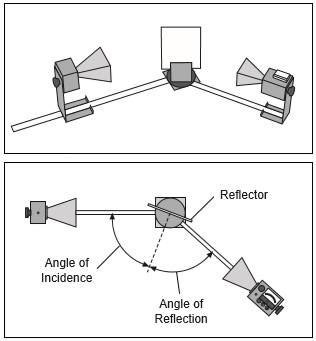
\includegraphics[width=0.7\linewidth]{Pictures/reflexion}
\caption{Montaje experimental - Refelxión de Microondas}
\label{fig:reflexion}
\end{figure}

A continuación, dejando el emisor de ondas fijo, a un ángulo de $45^o$ con respecto a la normal del reflector, se procedió a mirar para qué ángulo el receptor mostraba una señal máxima. Se encontró que $45^o$ era el máxmimo de la señal. Esto se hizo para verificar el montaje. \\

Acto seguido, la intensidad del receptor se ajustó en 30X para asegurarse de detectar las más pequeñas variaciones, y se procedió a mover el ángulo incidente desde $20^o$ a $90^o$. El receptor se movió angularmente hasta detectar un máximo. De allí se pudo inferir la relación entre el ángulo incidente y el ángulo reflejado.  \\

Debe anotarse que dado que las ondas son esféricas, hay una medición extra dado que la onda recibida por detector no es sólamente la reflejada sino también se suma una porción directamente proveniente del emisor.\\

\subsection{\label{sec:level2}Refracción a través de un prisma}

Para esta manipulación se configuró el montaje mostrado en la figura \ref{fig:refraccion}. El compartimiento triangular del centro actuaba como prisma. \\

\begin{figure}[h!]
\centering
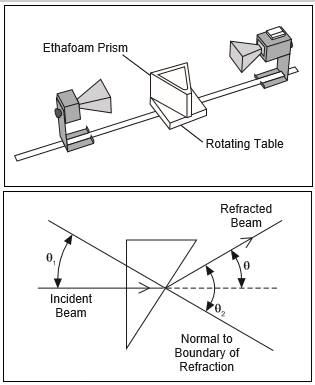
\includegraphics[width=0.7\linewidth]{Pictures/refraccion}
\caption{Montaje Experimental - Refracción por prisma}
\label{fig:refraccion}
\end{figure}
 
En primer lugar, se procedió a determinar la influencia de este material en la señal del receptor y una vez demostrado que la diferencia era prácticamente nula, se rellenó el interior del prisma con partículas de estireno.\\ 

Con el emisor de ondas fijo, se procedió a mover el detector hasta detectar un máximo en la señal.  Se denota, $ \theta $ el ángulo que marca directamente el detector con el goniómetro. \\

Una vez hallado este ángulo, con el diagrama de la figura \ref{fig:refraccion} se pueden determinar los ángulos incidente y refractado y así hallar el coeficiente de refracción del estireno por medio de la Ley de Snell. \\

En este caso, el medio incidente es el estireno.\\
 
\subsection{\label{sec:level2}Polarización}

Este experimento tuvo dos partes. En primer lugar, el montaje consistía en el que se muestra en la figura \ref{fig:polarizador1} con la excepción de que no había una rejilla de polarización en el medio. Con esto, receptor y emisor frente a frente se procedió a mover el cuerno del detector de ondas dejando el receptor fijo. De esta manera, las ondas producidas impactarían el detector con diferentes ángulos de polarización. \\ 

\begin{figure}[h!]
\centering
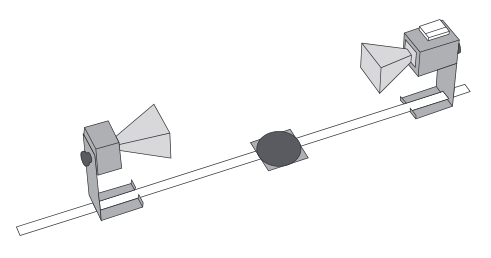
\includegraphics[width=0.7\linewidth]{Pictures/polarizador1}
\caption{Montaje Experimental - Polarización}
\label{fig:polarizador1}
\end{figure}

Se midieron así, en aumentos de $5^o$ las señales recibidas para un rango de ángulos de polarización entre $0^o$ y $90^o$. \\

En la segunda parte se prepararon el emisor y el receptor con direcciones paralelas de polarización, se incluyó la rejilla de polarización imitando el montaje en la figura \ref{fig:polarizacion}, y ésta se ubicó en ángulo de $0^o$,$22.5^o$,$45^o$, $67.5^o$ y $90^o$ con respecto al ángulo del emisor. Luego se  se repitieron las medidas para $0^o$, $45^o$ y $90^o$, esta vez configurando el emisor y el receptor en direcciones perpendiculares de polarización.\\ 

\begin{figure}[h!]
\centering
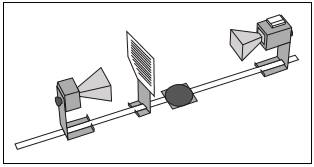
\includegraphics[width=0.7\linewidth]{Pictures/polarizacion}
\caption{Montaje Experimental - Polarización 2}
\label{fig:polarizacion}
\end{figure}

\subsection{\label{sec:level2}Determinación de $ \lambda $}
\textit{Interferencia de doble rendija} \\

\begin{figure}[h!]
\centering
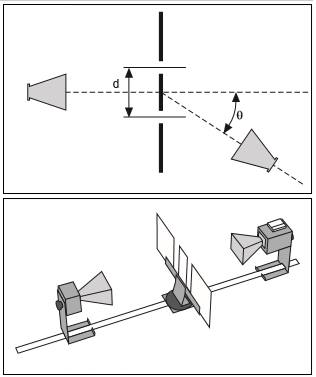
\includegraphics[width=0.7\linewidth]{Pictures/Interferencia}
\caption{Montaje Experimental - Interferencia a Doble Rendija}
\label{fig:Interferencia}
\end{figure}

En este experimento se armó el montaje mostrado en la figura \ref{fig:Interferencia}. Dejando el emisor de ondas fijo, se movió el detector a través del ángulo $ \theta $ mostrado en la figura. Para un barrido de este ángulo entre $0^o$ y $85^o$ en aumentos de $5^o$, se anotó el valor de la intensidad detectada por el receptor. \\

Se repitieron las medidas cambiando la distancia de separación entre rendijas.\\ 

\textit{Ondas estacionarias} \\

Para medir ondas estacionarias se utilizó como reflector el detector mismo. Se ubicaron frente a frente ambos equipos como se muestra en la figura \ref{fig:estacionarias}. \\

\begin{figure}[h!]
\centering
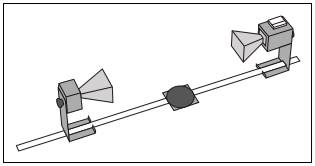
\includegraphics[width=0.7\linewidth]{Pictures/estacionarias}
\caption{Montaje Experimental - Ondas estacionarias}
\label{fig:estacionarias}
\end{figure}

A continuación, se ubicó el detector en donde éste mostrara la lectura de un máximo, y acto seguido se procedió a deslizar el detector hacia atrás. En dos manipulaciones diferentes, se contaron 20 y 30 máximos respectivamente y se procedió a determinar $ \lambda $ con la fórmula para los máximos de una onda estacionaria, la cual es la misma condición presentada en la ecuación \ref{eq:Michelson}. \\ 

\textit{Espejo de Lloyd} \\

Para determinar $ \lambda $ se utilizó también el montaje del espejo de Lloyd mostrado en la figura \ref{fig:espejo}. En este caso el receptor mostrará una señal máxima cuando ambos caminos recorridos por la onda emitida estén en fase. \\

\begin{figure}[h!]
\centering
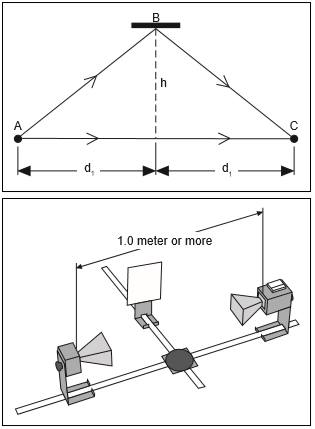
\includegraphics[width=0.7\linewidth]{Pictures/espejo}
\caption{Montaje Experimental - Espejo de Lloyd}
\label{fig:espejo}
\end{figure}

Para medir este fenómeno se dejan reflector y emisor fijos, separados a una distancia idéntica desde el centro del sistema y se desplaza el reflector hacia atrás. \\

En primer lugar, debe ubicarse el reflector en el primer mínimo que sea posible detectar y acto seguido desplazarlo hacia atrás hasta encontrar cuando menos 10 mínimos de intensidad. De esta forma, la diferencia de caminos debe cumplir la ecuación \ref{eq:Lloyd} para producir interferencia constructiva\\

La medición se realizó dos veces para diferentes separaciones entre emisor y receptor.\\


\textit{Interferómetro de Fabry-Perot} \\

En este caso se recreó el interferómetro de Fabry-Perot, haciendo uso del montaje mostrado en la figura \ref{fig:fabryperot}. Durante esta manipulación se pretendía encontrar la longitud de onda así que se procedió de manera similar al experimento de ondas estacionarias y al espejo de Lloyd.\\


\begin{figure}[h!]
\centering
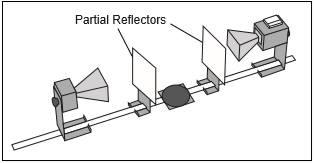
\includegraphics[width=0.7\linewidth]{Pictures/fabryperot}
\caption{Montaje Experimental - Interferómetro de Fabry-Perot}
\label{fig:fabryperot}
\end{figure}

Dejando el emisor fijo se ubicó el receptor en un mínimo. Acto seguido, se procedió a mover el mismo hacia atrás hasta haber pasado por n mínimos de intensidad. Así pues, con la fórmula \ref{eq:Michelson}, se determinó la longitud de onda. \\ 

\textit{Interferómetro de Michelson} \\

En este experimento se trató de recrear el experimento de Michelson-Morley con microondas, haciendo uso del montaje mostrado en la figura \ref{fig:intmichelson}. \\

\begin{figure}[h!]
\centering
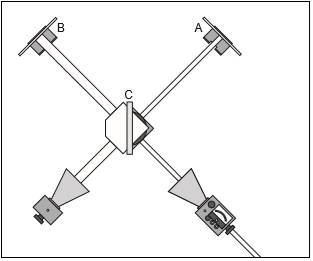
\includegraphics[width=0.7\linewidth]{Pictures/intmichelson}
\caption{Montaje Experimental - Interferómetro de Michelson}
\label{fig:intmichelson}
\end{figure}

Se ubicó el detector en el mínimo más cercano encontrado con respecto al centro del sistema y se procedió a deslizar el equipo hacia atrás contando mínimo diez mínimos de intensidad. Con una fórmula similar a las utilizadas anteriormente, se determinó $ \lambda $. \\

La fórmula utilizada es la misma que para el interferómetro de Fabry-Perot. \\


\subsection{\label{sec:level2}Fibra Óptica}

Para el experimento de fibra óptica se utilizaron nuevamente las partículas de estireno, sólo que en esta ocasión se configuró una suerte de fibra óptica al ponerlas de relleno en una bolsa larga de plástico. \\

El experimento es de énfasis cualitativo y consistió en estudiar cómo, por medio de la fibra óptica, el detector puede leer la intensidad de la onda incidente en diferentes configuraciones. \\

Dichas configuraciones consistían en mover el cuerno del emisor y el receptor cambiando el ángulo de polarización como también ver cómo cambiaba la señal al cambiar la curvatura de la fibra. \\ 

Se quería comprobar también que si uno de los extremos no se encontraba debidamente introducido en los cuernos de los equipos, la lectura sería cero. \\


\section{\label{sec:level1}Resultados y An\'alisis}

\subsection{\label{sec:level2}Radiación de fondo}
En este experimento medimos la radiación de fondo promedio. Tomamos 5 datos de 60 segundos cada uno, los cuales se encuentran registrados en la tabla \ref{table:fondo}.\\

\begin{table}[h!]
\centering
\begin{tabular}{|c|}
	\hline $ Conteo (\pm 1) $ \\ 
	\hline\hline
	27\\
	20\\
	16\\
	19\\
	24\\
	[1ex] 
 \hline
 \end{tabular} 
  \caption{Radiación ambiental}
\label{table:fondo} 
\end{table}

El objetivo de este experimento era verificar si se podía detectar radiación en ausencia de una muestra. Esta radiación detectada la llamamos radiación de ambiente y se debe a decaimientos espontáneos de isótopos radiactivos en la materia que nos rodea; a la radiación cósmica de fondo y a las muestras de radiación que se encontraban en mesas cercanas. Las muestras que se encontraban en dichas mesas variaban constantemente su ubicación y su nivel de radiactividad dependía de los experimentos que otros estuvieran haciendo, por lo cual era conveniente medir la radiación de fondo al realizar cada montaje.\\

Esta radiación de fondo tiene como promedio un valor de $0.353$ conteos por segundo. En estas mediciones, debido al caracter probabilístico de su naturaleza, una buena medida del error es la desviación estándar. A lo largo de este informe escogemos la definición de error absoluto asociado a su medida como tres veces su desviación estándar. Esta medida, $\delta x = 3\sigma_x$ tiene un $99.7\%$ de confianza, es decir, cada medida tiene  $99.7\%$ de probabilidad de estar en el rango dado por dicho error. En este caso, la media, incluyendo su error absoluto está dada por $C = 0.353 \pm 0.193\frac{cts}{s}$. Esta medida de error, es cada vez más confiable entre más medidas tengamos, dado que la desviación estandar real asociada a la distribución de probabilidad del fenómeno se obtiene, por definición, sobre un número infinito de realizaciones de dicha distribución. Podemos ver la veracidad de este factor dado que en este caso obtuvimos un error relativo bastante grande para solo 5 medidas: $54\%$.\\

\subsection{\label{sec:level2}Variaciones} 
En este experimento verificamos la naturaleza estadística de la radiación al tomar 50 medidas de 10 segundos sobre una manta incandescente.\\

La distribución de probabilidad que mejor caracteriza el proceso estocástico de decaimiento de s radiactivos es la distribución de Poisson. Esta distribución tiene como característica que su varianza es igual a su promedio, y en términos de la desviación estándar: $\sigma_x^2 = \bar{x}$. Debido a que esta distribución es discreta, hacer cálculos de intervalos de confianza resulta difícil, sin embargo, podemos aproximar su forma de campana como una Gaussiana. En este sentido, se tiene que el $68.27\%$ de los datos estarán concentrados alrededor del promedio con radio igual a una desviación estándar. Si se escoje un radio de $2\sigma$, $95.45\%$ de los datos estarán concentrados en el intervalo, y si se tienen $3\sigma$ (el error absoluto definido para este informe), se tendrá una confianza del $99.73\%$.\\

Teniendo los anteriores datos en cuenta, se puede notar que el porcentaje de error debido a la definición $\delta x = 3\sigma_x$ está dado por $\epsilon = \frac{3\sigma_x}{\bar{x}} = \frac{3}{\bar{x}}$. Esto evidencia la importancia del tiempo en las medidas que tomamos, ya que si se toman conteos por un intervalo de tiempo mayor, el promedio será claramente mayor, y por tanto, el error relativo disminuirá. Además de esto, con esta propiedad es posible estimar el error asociado a una medida sin tener una muestra estadistica significativamente grande.\\


Sin más preámbulos, los datos obtenidos se encuentran consignados en la tabla \ref{table:variaciones} y un histograma donde se pueden apreciar claramente las características de una distribución de Poisson con baja resolución, se encuentra graficado en la figura \ref{fig:variaciones}.\\

\begin{table}[h!]
\centering
\begin{tabular}{|c|c|c|c|}
	\hline $ N^oMedicion $ & $Resultado(\pm 1)$ & $ N^oMedicion $ & $Resultado(\pm 1)$ \\ 
	\hline\hline
	1&65&26&66\\
	2&63&27&73\\
	3&57&28&60\\
	4&67&29&59\\
	5&67&30&82\\
	6&78&31&74\\
	7&67&32&72\\
	8&56&33&62\\
	9&78&34&66\\
	10&55&35&57\\
	11&80&36&75\\
	12&69&37&56\\
	13&61&38&79\\
	14&70&39&65\\
	15&68&40&68\\
	16&65&41&75\\
	17&69&42&67\\
	18&58&43&71\\
	19&71&44&73\\
	20&75&45&65\\
	21&61&46&69\\
	22&73&47&70\\
	23&54&48&64\\
	24&79&49&56\\
	25&64&50&64\\	
		[1ex] 
 \hline
 \end{tabular} 
  \caption{Variación estadística}
\label{table:variaciones} 
\end{table}


\begin{figure}[h!]
\centering
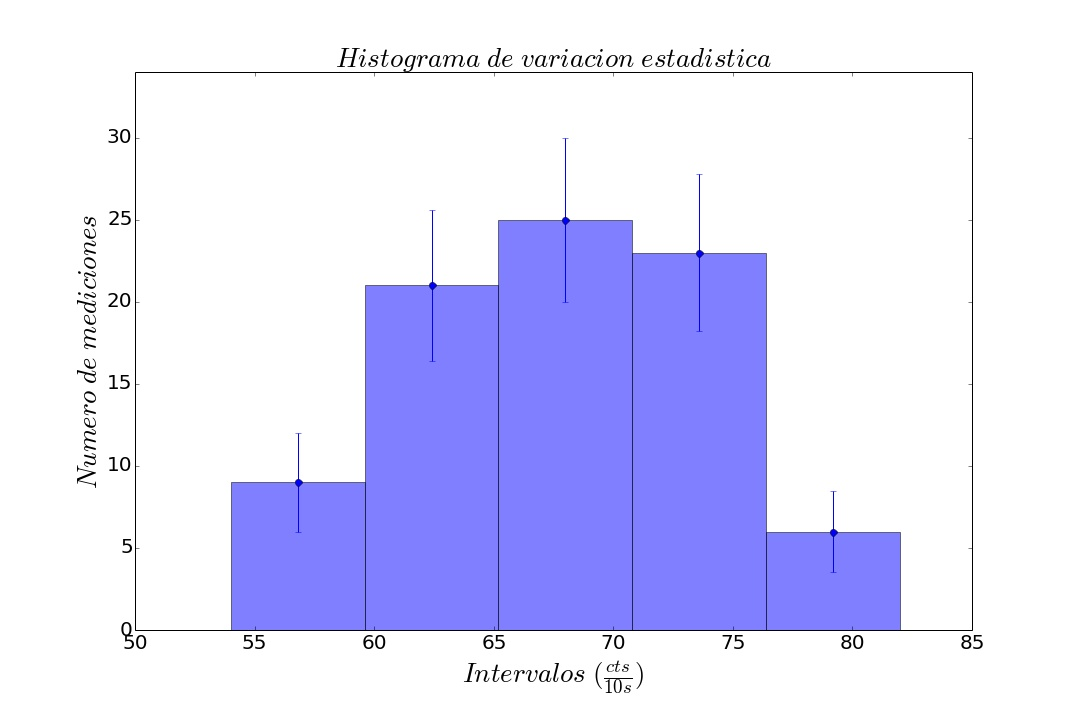
\includegraphics[width=0.8\linewidth]{variacion.jpg}
\caption{Histograma de los conteos medidos}
\label{fig:variaciones}
\end{figure}

En este experimento se obtuvo un promedio de 67.16 conteos cada 10 segundos, y una desviación estándar de    7.19 en las mismas unidades. Nótese que la raiz cuadrada del promedio debería ser igual a la desviación estándar si la distribución estudiada es de Poisson. En este caso dicha raiz es de 8.19, que comparada con el valor real, presenta un error de solo $12\%$, lo cual es bastante razonable para un análisis estadístico.\\

Ahora, al verificar el intervalo de confianza que provoca una desviación estándar, descubrimos que el $64\pm2\%$ de los datos se encontraban en dicho intervalo, lo cual muestra un error de 6.25\% con el valor esperado de $68\%$.\\

Los errores obtenidos en este montaje son naturales de la calidad estocástica de los procesos involucrados. En principio, para los análisis estadísticos siempre necesitaremos una cantidad infinita de mediciones para obtener conclusiones exactas. A pesar de dichos errores, pudimos identificar la distribución de probabilidad de las medidas como una distribución de Poisson.\\

\subsection{\label{sec:level2}Radiactividad en sales} 
En esta sección verificamos si las muestras de sales $CaCl$, $Cu_2SO_4$, $NaCl$, $KCl$ emitían radiación ionizante. Para ello medimos cuatro veces los conteos que provocaban en el contador Geiger duratnte 60 segundos, y los comparamos con la radiación del ambiente.\\

Los datos obtenidos se encuentran consignados en la tabla \ref{table:sales}.\\

\begin{table}[h!]
\centering
\begin{tabular}{|c|c|c|c|c|c|c|}
	\hline $ Muestra $ & \multicolumn{4}{c|}{$Resultado\ (\pm 1)$ } & $\bar{x}$& $\sigma_x$ \\ 
	\hline\hline
	CaCl2&28&22&21&22&23.25&2.77\\
	Cu2SO4&21&15&32&16&21.0&6.75\\
	KCl&43&41&44&34&40.5&3.91\\
	NaCl&25&23&23&16&21.75&3.42\\
	Ambiente&23&23&23&15&21.0&3.46\\
	[1ex] 
 \hline
 \end{tabular} 
  \caption{Radiación por diferentes muestras de sales}
\label{table:sales} 
\end{table}

De esta tabla, teniendo en cuenta las desviaciones estándares, se puede concluir el cloruro de potasio es claramente radiactivo ya que, teniendo en cuenta el error estadístico, su intervalo no cae en la radiación ambiente; el cloruro de calcio es posiblemente radiactivo ya que, aunque su promedio es mayor, hay una pequeña intersección entre su intervalo de confianza y el de la radiación de ambiente; y el resto de sales, cloruro de sodio y sulfato de cobre, no presentan una diferencia significativa con la radiación de ambiente para tener una conclusión convinvcente.\\

\subsection{\label{sec:level2}Radiactividad en rocas} 
Al igual que en la sección anterior, verificamos radiactividad esta vez en rocas en lugar de sales. Para esto, hicimos las mismas 4 mediciones de 60 segundos sobre cada una de las muestras y sobre el ambiente. Las rocas utilizadas en este experimento contenían cada una, y por separado, restos de Ba-133, de Cd-109 y Cs-137.\\

Los datos tomados se encuentran en la tabla \ref{table:rocas}.\\

\begin{table}[h!]
\centering
\begin{tabular}{|c|c|c|c|c|c|c|}
	\hline $ Muestra $ & \multicolumn{4}{c|}{$Resultado\ (\pm 1)$ } & $\bar{x}$& $\sigma_x$ \\ 
	\hline\hline
	Ba-133&611&639&607&642&624.75&15.85\\
	Cd-109&81&67&66&70&71.0&5.96\\
	Cs-137&3279&3198&3146&3186&3202.25&48.31\\
	Ambiente&24&20&24&22&22.6&1.66\\
	[1ex] 
 \hline
 \end{tabular} 
  \caption{Radiación por diferentes muestras de rocas}
\label{table:rocas} 
\end{table}

En este caso encontramos que todas las rocas medidas eran radiactivas. Claramente la más activa era la de Cesio, seguida de la de Bario y de la de Cadmio. Todas las muestras tuvieron promedios superiores a la radiación ambiente, con varianzas que permitían admitir con certeza que eran radiactivas. Las varianzas pequeñas registradas en comparación con las medidas evidencia una vez más que la distribución de Poisson rige estos decaimientos radiactivos.\\

\subsection{\label{sec:level2}Diferentes tipos de radiacion en Columbita}
En este experimento medimos diferentes tipos de radiación al poner diferentes filtros a una roca de columbita. Para esto, medimos 3 conteos en intervalos de 100 segundos para la roca de frente y de revés. Luego tomamos las mismas medidas para el lado más radiactivo de la roca superponiendo filtros de papel y aluminio. Claramente no faltó la medición de la radiación ambiente.\\

Los datos de radiación ambiente se encuentran consignados en la tabla \ref{table:ambiente5}. Mientras los datos de radiación con diferentes filtros de columbita se encuentran en la tabla \ref{table:columbita}.\\


\begin{table}[h!]
\centering
\begin{tabular}{|c|c|}
	\hline $Medicion $ & $ Conteo (\pm 1) $ \\ 
	\hline\hline
	1&42\\
	2&32\\
	3&34\\
	4&36\\
	5&41\\
	Prom&37.0\\
	Std&3.90\\
	[1ex] 
 \hline
 \end{tabular} 
  \caption{Radiación ambiental}
\label{table:ambiente5} 
\end{table}


\begin{table}[h!]
\centering
\begin{tabular}{|c|c|c|c|c|c|}
	\hline $ Muestra $ & \multicolumn{3}{c|}{$Resultado\ (\pm 1)$ } & $\bar{x}$& $\sigma_x$ \\ 
	\hline\hline
	No Filtro 1 &326&349&318&331.0&13.14\\
	Papel 1&329&355&344&342.67&10.67\\
	Metal 1&146&187&160&164.33&17.02\\
	No Filtro 2 &286&321&286&297.67&16.50\\
	[1ex] 
 \hline
 \end{tabular} 
  \caption{Distintos filtros para la Columbita}
\label{table:columbita} 
\end{table}

De esta tabla es importatne notar que la radiación de ambiente es prácticamente insignificante respecto a las radiaciones obtenidas incluso con los filtros, y para los objetivos de esta sección no es importante tenerla en cuenta, ya que no realizaremos ningún cálculo, solo compararemos los promedios y varianzas.\\

Así, es sencillo notar que la diferencia entre los conteos realizados cuando se tenía el lado más radiactivo de la columbita respecto a la misma situación con un filtro de papel, son prácticamente insignificantes dadas las varianzas. Esto nos permite afirmar con bastante certeza que la radiación emitida por la columbita no está compuesta de radiación $\alpha$ o su fracción es muy pequeña para ser medida por este experimento. \\

Por otro lado, los conteos del filtro metálico son claramente menores que los conteos normales sin filtro. A su vez, estos son significativamente mayores que la radiación ambiente por varias desviaciones estándares. Esto nos permite afirmar que mucha de la radiación emitida por la columbita es radiación $\beta$, casi la mitad, mientras la otra mitad, al poder atravesar el filtro de metal, se compone de radiación $\gamma$. Si sustraemos la radiación ambiente de los conteos con los filtros y sin ellos podremmos dar un estimado de la proporción de radiación de tipo $\beta$ y $\gamma$ que emite la columbita.\\

Así, la columbita produce en promedio un valor total de $294 \pm 13.14$ conteos cada 100 segundos, mientras que con el filtro de metal produce $127.33 \pm 17.02$. Omitiendo las varianzas y asumiendo que el filtro de metal para completamente la radiación $\beta$, la proporción de radiación $\beta$ y $\gamma$ es de respectivamente de $56.67 \pm 0.06\%$  y de $43.33 \pm 0.06\%$. Aquí los errores absolutos se calcularon con las respectivas propagaciones de error.\\

La composición de radiación $\beta$ de la roca se puede verificar cualitativamente porque al voltearla el número de conteos disminuyó. En este caso, la misma roca actuaba como un filtro no perfecto no tan poderos como el de metal que usamos, pero que de todas maneras reducía la radiación $\beta$ recibida por el contador.\\

\subsection{\label{sec:level2}Diferentes tipos de radiacion en manta incandescente}
En este experimento el objetivo era el mismo que en la sección anterior, esta vez, para una manta incandescente. Para lograr dicho objetivo tomamos 5 conteos en 60 segundos cada uno teniendo como objetivo la manta, la manta con un filtro de papel y luego de plomo, y el ambiente. Los datos obtenidos se encuentran en la tabla \ref{table:incandescente}.\\

\begin{table}[h!]
\centering
\begin{tabular}{|c|c|c|c|c|c|}
	\hline $ Medicion $ & $Manta$ & $Papel$ & $Metal$ & $Ambiente$ \\
	\hline\hline
	1&672&586&126&22\\
	2&696&573&148&28\\
	3&746&627&144&42\\
	4&691&608&149&21\\
	5&754&655&160&20\\
	Prom&711.80&609.80&145.40&26.60\\
	Var&32.30&29.19&11.06&8.19\\
		[1ex] 
 \hline
 \end{tabular} 
  \caption{Distintos filtros para la manta incandescente}
\label{table:incandescente} 
\end{table}

De esta tabla es importante notar que no hay preocupaciones por las mediciones respecto al ambiente. En cada caso las medidas fueron claramente diferentes entre ellas y con el ambiente por varias desviaciones estándares. Dada esta diferencia clara entre los conteos con diferentes filtros y respecto al ambiente, podemos afirmar con gran certeza que la manta incandescente emite radiación compuesta por rayos $\alpha$, $\beta$ y $\gamma$.\\

Sabiendo que los rayos $\alpha$ solo son parados por papel y metal, que los rayos $\beta$ solo son parados por metal, y que los rayos $\gamma$ son imparables por papel y metal, podemos obtener un valor para las fracciones de composición de la radiación de la manta. Sin embargo, para que estas fracciones no se vean alteradas por el ambiente, es necesario restar su contribución a cada medida.\\

De esta manera tenemos que la manta provoca en 60 segundos um promedio de $685.2\pm32.3$ conteos, mientras que la misma medida con filtros de papel y metal son, en promedio, respectivamente $583.2\pm29.19$ y $118.8\pm11.06$. Con estos datos, y la información en el párrafo anterior podemos concluir que la radiación ionizante emitida por la manta incandescente se compone en un $14.89\pm0.05\%$ de rayos $\alpha$, en un $67.78\pm0.05\%$ de rayos $\beta$ y en un $17.34 \pm0.018\%$ de rayos $\gamma$.\\

Aquí vemos que la manta incandescente emite todos los tipos de radiación, $\alpha$, $\beta$ y $\gamma$. Ahora, dado que la radiación $\beta$ y $\alpha$ no puede ser emitida en un mismo proceso atómico, los resultados de este experimento demuestran que la manta incandescente contiene materiales reactivos que emiten radiación por al menos 2 procesos atómicos.\\

\subsection{\label{sec:level2}Dependencia de la intensida de radiación con la distancia}
En este experimento pretendíamos medir la dependencia de la intensidad de radiación con la distancia de la fuente. Para ello, tomamos conteos de 10 segundos de una muestra de Ra-226 a distancias desde 2cm hasta 10cm equiespaciadas a 1cm. Además, se duplicó el experimento con medidas de 10 segundos una muestra del mismo elemento, esta vez, mucho más radiactiva. Los datos obtenidos se encuentran en la tabla \ref{table:distancia} y \ref{table:fuerte}.\\


\begin{table}[h!]
\centering
\begin{tabular}{|c|c|c|c|c|c|c|c|}
	\hline $D(\pm0.1cm)$& $c_1(\pm1)$ & $c_2(\pm1)$ & $c_3(\pm1)$& $c_4(\pm1)$& $c_5(\pm1)$& $\bar{c}$ & $\sigma_c$\\
	\hline\hline
	2 & 539 & 530 & 536 & 553 & 554 & 542.4 & 9.5\\
	3 & 278 & 283 & 294 & 281 & 269 & 281.0 & 8.0\\
	4 & 173 & 183 & 184 & 166 & 190 & 179.2 & 8.5\\
	5 & 123 & 139 & 134 & 112 & 129 & 127.4 & 9.4\\
	6 & 99  & 104 & 100 & 77  & 105 & 96.8  & 10.1\\
	7 & 93  & 76  & 78  & 82  & 65  & 78.8  & 9.1\\
	8 & 68  & 70  & 72  & 66  & 77  & 70.6  & 3.8\\
	9 & 67  & 55  & 48  & 67  & 65  & 60.4  & 7.6\\
	10& 45  & 40  & 52  & 48  & 64  & 49.8  & 8.1\\
	[1ex] 
 \hline
 \end{tabular} 
  \caption{Dependencia de la radiación con la distancia (Ra-226 débil)}
\label{table:distancia} 
\end{table}

\begin{table}[h!]
\centering
\begin{tabular}{|c|c|c|}
	\hline $D(\pm0.1cm)$& $c(\pm1)$& $\sigma_c$\\
	\hline\hline
	4.00&8558&92.51\\
	5.00&5281&72.67\\
	6.00&3899&62.44\\
	7.00&3089&55.58\\
	8.00&2376&48.74\\
	9.00&1993&44.64\\
	10.00&1563&39.53\\
	11.00&1303&36.10\\
	12.00&1074&32.77\\
	[1ex] 
	\hline
 \end{tabular} 
  \caption{Dependencia de la radiación con la distancia (Ra-226 fuerte)}
\label{table:distancia} 
\end{table}

Debido al poder de la segunda fuente utilizada, no necesitamos un fuerte respaldo estadístico, ya que según la distribución de Poisson, el error relativo disminuye con el inverso de la raiz del promedio (en este caso la medida). Así, solo tomamos una medida de 10 segundos y tomamos la raiz cuadrada de dicho valor como error. Cabe resaltar que para $d= 2cm$ y $d = 3cm$ en la muestra fuertemente radiactiva, el contador se saturaba, por lo que no tomamos estos conteos.\\

Para poder analizar la dependencia de la intensidad con la distancia de una mejor manera, se obtuvieron gráficas para cada muestra. Ahora, como normalmente sucede, la intensidad de una fuente depende inversamente del cuadrado de la distancia a la que está el detector. Por esto, teniendo en cuenta que la intensidad es proporcional al número de conteos, se hizo un ajuste de la forma:\\

\begin{equation}
 	C(d) = A + \frac{B}{d^2}
\end{equation}

Donde $A$ corresponde a la intensidad percibida e invariante del ambiente, y B corresponde a una constante de calibre  para la dependencia de la fuente de radio con la distancia. En el caso del Ra-226 fuerte el efecto del ambiente es sumamente insignificante, por lo cual se tomó $A = 0$.\\

Los resultados de los ajustes, así como sus respectivas gráficas se encuentran en las figuras \ref{fig:distancia} y \ref{fig:cuadrados}.\\

\begin{figure}[h!]
\centering
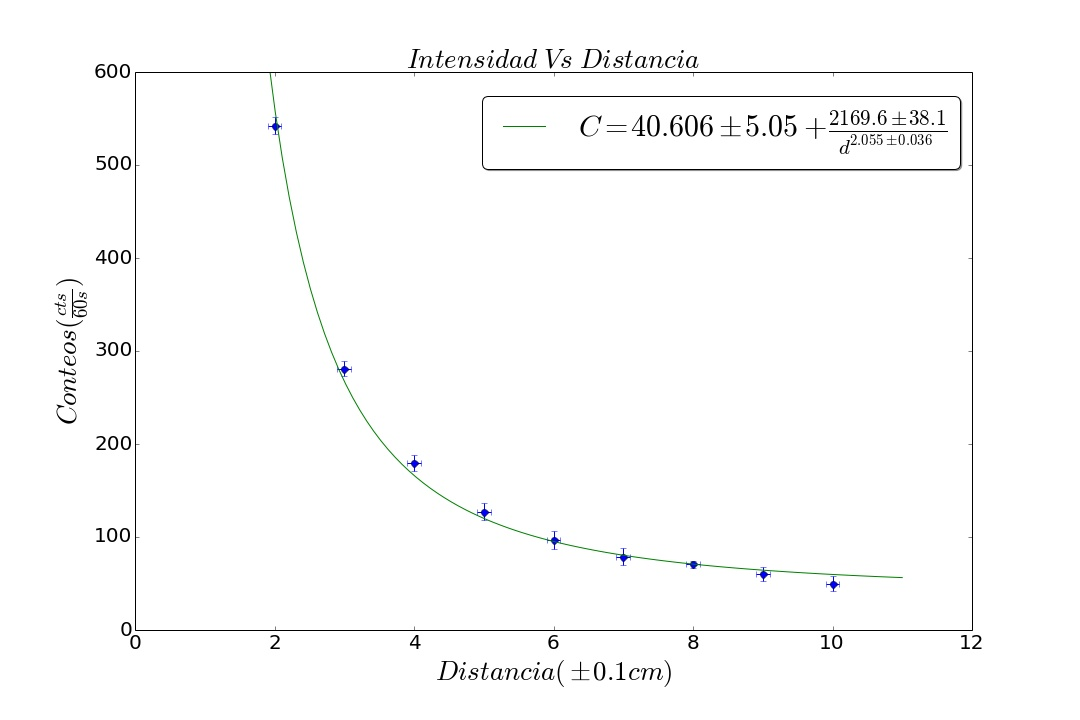
\includegraphics[width=1.1\linewidth]{distancia.jpg}
\caption{Relación de intensidad con la distancia a la fuente (Ra-226 débil)}
\label{fig:distancia}
\end{figure}

\begin{figure}[h!]
\centering
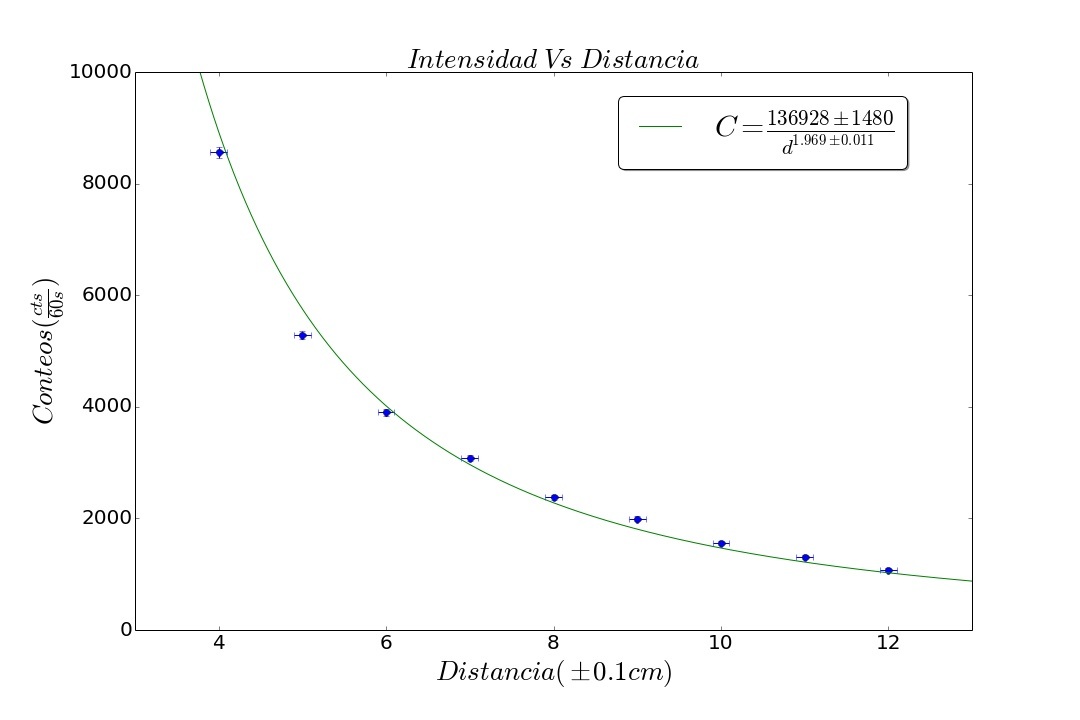
\includegraphics[width=1.1\linewidth]{cuadrados.jpg}
\caption{Relación de intensidad con la distancia a la fuente (Ra-226 fuerte)}
\label{fig:cuadrados}
\end{figure}

Dicho ajuste verifica la relación cuadrática de la intensidad con la distancia a la fuente. El valor del exponente es de $2.055\pm0.036$  para la fuente débil y de $1.969\pm0.011$ lo cual solo está alejado de la realidad un 2.75\% y un 1.5\%. La diferencias de errores se debe a la propagación de los errores relativos, los cuales son menores para conteos muy grandes.\\

Con esto concluimos que la intensidad de radiación decae inversamente con el cuadrado de la distancia a la fuente, independientemente de la fuente utilizada.\\
 
\subsection{\label{sec:level2}Rango de la radiación alpha}
En esta sección evaluamos el alcance de la radiación $\alpha$ emitida por una muestra de Ra-226. Para ello tomamos conteos durante 10 segundos variando la distancia sobre la muestra sin filtro, y la muestra con un filtro de papel. Los datos obtenidos se pueden apreciar en la tabla \ref{table:alcance}.\\

\begin{table}[h!]
\centering
 \begin{tabular}{|c|c|c|c|c|} 
 \hline
 $Distancia(\pm0.1cm)$& $C_{filtro}(\pm1)$& $\delta_{filtro}$ & $C_{0}(\pm1)$ & $\delta_0$ \\ [0.5ex] 
 \hline\hline
 3.00&5299&72.79&13640&116.79\\
 3.50&4225&65.00&11030&105.02\\
 4.00&3406&58.36&9570&97.83\\
 4.50&2722&52.17&7124&84.40\\
 5.00&2394&48.93&5740&75.76\\
 5.50&2106&45.89&4985&70.60\\
 6.00&1765&42.01&4230&65.04\\
 6.50&1558&39.47&3706&60.88\\
 7.00&1361&36.89&3163&56.24\\
 7.50&1159&34.04&2755&52.49\\
 8.00&1046&32.34&2500&50.00\\
 8.50&940&30.66&2258&47.52\\
 9.00&825&28.72&1989&44.60\\
 9.50&795&28.20&1841&42.91\\
 10.00&710&26.65&1652&40.64\\
 11.00&595&24.39&1369&37.00\\
 12.00&553&23.52&1098&33.14\\
 13.00&461&21.47&967&31.10\\
 14.00&334&18.28&818&28.60\\
 15.00&299&17.29&680&26.08\\
 16.00&288&16.97&582&24.12\\
 17.00&217&14.73&494&22.23\\
 18.00&205&14.32&417&20.42\\
 20.00&144&12.00&320&17.89\\
 25.00&97&9.85&189&13.75\\
 [1ex] 
 \hline
 \end{tabular}
 \caption{Mediciones de Ra-226 con y sin filtro de papel}
 \label{table:alcance}
\end{table}

Cabe resaltar que la fuente tomada era sumamente radiactiva y para distancias muy cortas el contador se saturaba, por lo se omitieron dichas medidas. Además, dado que no se tomaron muchas medidas se tomó como error absoluto la raiz cuadrada de las medidas, lo cual es una buena aproximación teniendo en cuenta la distribución de Poisson que caracteriza los decaimientos.\\

Ahora, para verificar el alcance de la radiación $\alpha$, tenemos que obtener en qué fracción se reduce la radiación total al imponer el filtro a diferentes distancias. Dicha fracción corresponde a la fracción  de rayos $\alpha$ en la radiación total. Cuando la fracción reducida sea significativamente pequeña, podemos decir que la radiación $\alpha$ llegó a su límite de distancia recorrida. En la tabla \ref{table:fraccion} se pueden apreciar las diferencias de radiación para cada distancia, así como la fracción que esta diferencia representa respecto a la radiación sin filtro. Los errores expuestos fueron calculados con la respectiva propagación de error tomando los errores de Poisson ya mencionados.\\ 

\begin{table}[h!]
\centering
 \begin{tabular}{|c|c|c|c|} 
 \hline
 $Distancia(\pm0.1cm)$& $\Delta C$& $Fraccion\ Reducida$ & $\delta_{frac}$ \\ [0.5ex] 
 \hline\hline
3.00&8341&0.612&0.006\\
3.50&6805&0.617&0.007\\
4.00&6164&0.644&0.007\\
4.50&4402&0.618&0.009\\
5.00&3346&0.583&0.010\\
5.50&2879&0.578&0.011\\
6.00&2465&0.583&0.012\\
6.50&2148&0.580&0.013\\
7.00&1802&0.570&0.014\\
7.50&1596&0.579&0.015\\
8.00&1454&0.582&0.015\\
8.50&1318&0.584&0.016\\
9.00&1164&0.585&0.017\\
9.50&1046&0.568&0.018\\
10.00&942&0.570&0.019\\
11.00&774&0.565&0.021\\
12.00&545&0.496&0.026\\
13.00&506&0.523&0.027\\
14.00&484&0.592&0.027\\
15.00&381&0.560&0.031\\
16.00&294&0.505&0.036\\
17.00&277&0.561&0.036\\
18.00&212&0.508&0.042\\
20.00&176&0.550&0.045\\
25.00&92&0.487&0.064\\
 [1ex] 
 \hline
 \end{tabular}
 \caption{Fracciones de reducción de radiación por el filtro}
 \label{table:fraccion}
\end{table}

En esta tabla se puede apreciar que la fracción de radiación $\alpha$ parada por el filtro de papel no varió significativamente en las distancias medidas. A pesar de esto si se pudo notar una disminución generalizada de esta radiación alrededor de los 5cm. Después de dicha distancia la fracción no varió generalizadamente. \\

Ahora, debido a la interacción del aire con la radiación $\alpha$, esta no tiene mucho alcance dependiendo de su energía. Para el aire a presión constante y a $15^pC$, este alcance está dado por $D= 0.4769 E^{1.5}\frac{cm}{Mev}$. Si tenemos en cuenta la caida en la fracción de radiación $\alpha$, podemos encontrar que la muestra emitía dichos rayos con energías alrededor de $4.80 MeV$. Con un poco de investigación podemos intuir que dicha energía corresponde a la transición $Ra-226 \rightarrow Ra-222$, la cual es de $4.871Mev$. Si esta es, en efecto, la transición correcta, este método de cálculo de energía provoca únicamente un $2\%$ de error, congruente con los errores obtenidos anteriormente con estos montajes.\\

\subsection{\label{sec:level2}Influencia del grosor de los materiales en la radiación $\beta$}
En este experimiento medimos la influencia del grosor de materiales como el cartón, perspex y aluminio sobre la radiación $\beta$ de una fuente de Ra-226. Para ello tomamos diferentes medidas de conteo durante 10 segundos con la muestra a 3 cm del detector. Los datos obtenidos se encuentran en las tablas \ref{table:carton}, \ref{table:perspex} y \ref{table:aluminio}.\\

\begin{table}[h!]
\centering
 \begin{tabular}{|c|c|c|c|c|c|} 
 \hline
 $Grosor(\pm0.1cm)$ & $c_1(\pm1)$ & $c_2(\pm1)$ & $c_3(\pm1)$ & $\bar{c}$ & $\sigma_c$ \\ [0.5ex] 
 \hline\hline
 0.0&9936&9824&9849&9869.67&48.00\\
 0.5&1467&1428&1482&1459.00&22.76\\
 1.0&697&664&739&700.00&30.69\\
 1.5&363&364&324&350.33&18.62\\
 2.0&211&199&219&209.67&8.22\\
 2.5&162&165&143&156.67&9.74\\
[1ex] 
 \hline
 \end{tabular}
 \caption{Filtros de aluminio de diferente grosor}
 \label{table:aluminio}
\end{table}

\begin{table}[h!]
\centering
 \begin{tabular}{|c|c|c|c|c|c|} 
 \hline
 $Grosor(\pm0.1cm)$ & $c_1(\pm1)$ & $c_2(\pm1)$ & $c_3(\pm1)$ & $\bar{c}$ & $\sigma_c$ \\ [0.5ex] 
 \hline\hline
 0.0&9193&9194&9081&9156.00&53.03\\
 1.4&1468&1462&1541&1490.33&35.91\\
 2.8&608&652&583&614.33&28.52\\
 4.2&358&350&398&368.67&21.00\\
 5.6&271&222&230&241.00&21.46\\
[1ex] 
 \hline
 \end{tabular}
 \caption{Filtros de perspex de diferente grosor}
 \label{table:perspex}
\end{table}

\begin{table}[h!]
\centering
 \begin{tabular}{|c|c|c|c|c|c|} 
 \hline
 $Grosor(\pm0.1cm)$ & $c(\pm1)$ & $\delta_c$ \\ [0.5ex] 
 \hline\hline
 0.0&9207&95.95\\
 1.5&4359&66.02\\
 3.0&2554&50.54\\
 4.5&1765&42.01\\
 6.0&1284&35.83\\
 7.5&791&28.12\\
 9.0&699&26.44\\
 10.5&557&23.60\\
[1ex] 
 \hline
 \end{tabular}
 \caption{Filtros de carton de diferente grosor}
 \label{table:carton}
\end{table}

En estos casos, como error absoluto de las medidas con filtros de aluminio y perspex, se utilizó la desviación estándar; sin embargo, para el cartón debido a sus grandes conteos por su bajo poder de filtro, se tomó solo una medida y su error fue obtenido como la raiz cuadrada del valor medido. 

Ahora, la intensidad de radiación disminuye exponencialmente a través de un medio absorbente de la forma $I(d) = I_oe^{-\lambda d}$. Teniendo esto en cuenta, es necesario realizar un ajuste exponencial de esta forma, teniendo en cuenta la radiación ambiental como una constante aditiva. Dichos ajustes se encuentran representados en las figuras \ref{fig:aluminio}, \ref{fig:perspex} y ref{fig:carton}.\\


\begin{figure}[h!]
\centering
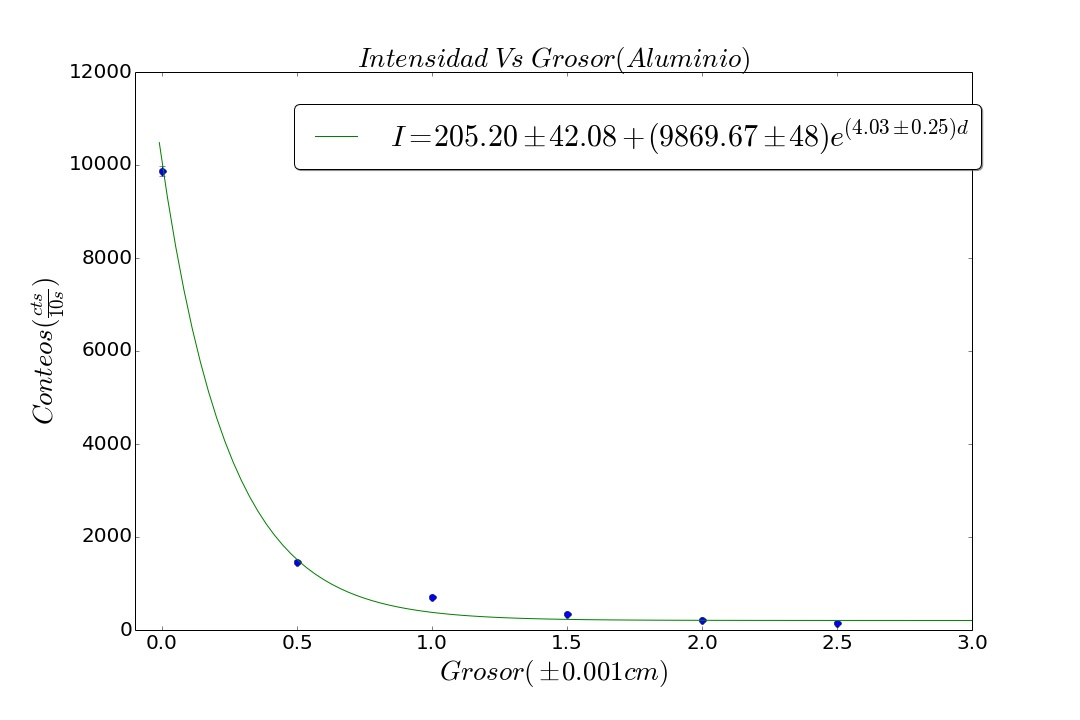
\includegraphics[width=1.1\linewidth]{aluminio.jpg}
\caption{Ajuste para la relació grosor-intensidad en el aluminio}
\label{fig:aluminio}
\end{figure}

\begin{figure}[h!]
\centering
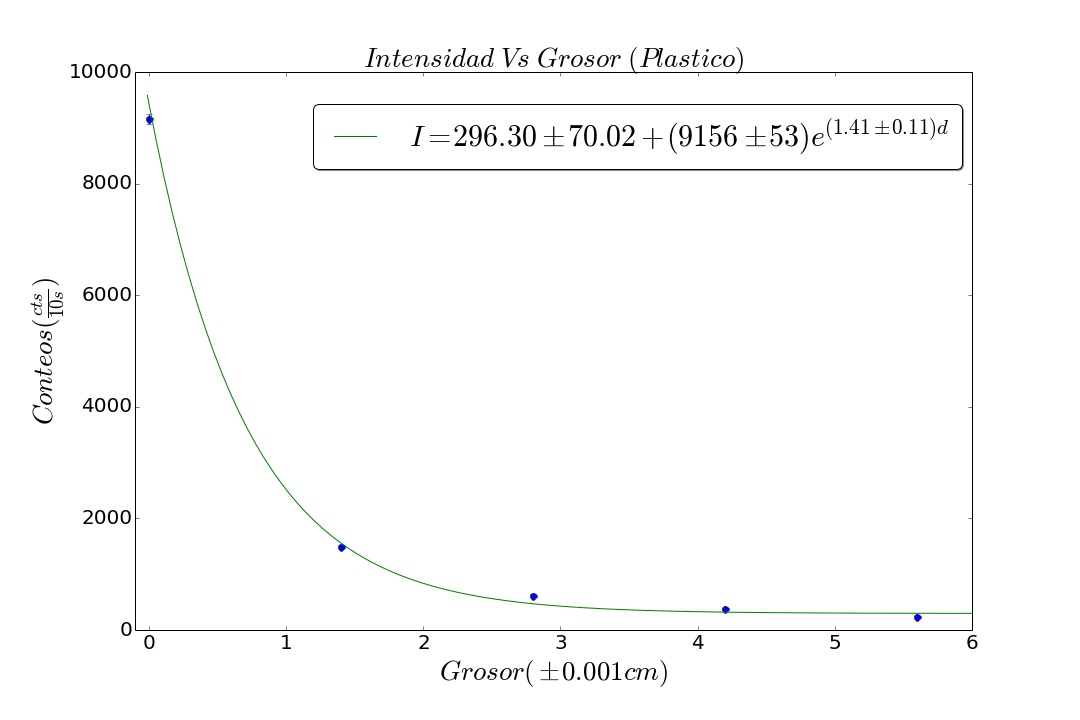
\includegraphics[width=1.1\linewidth]{perspex.jpg}
\caption{Ajuste para la relació grosor-intensidad en el perspex}
\label{fig:aluminio}
\end{figure}

\begin{figure}[h!]
\centering
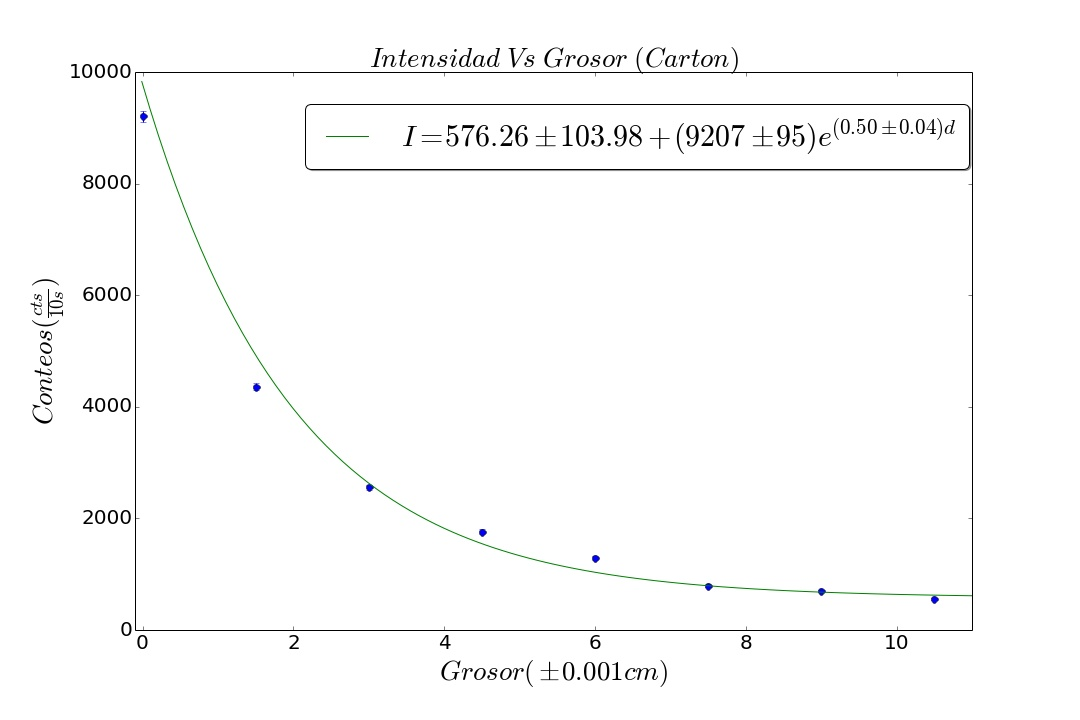
\includegraphics[width=1.1\linewidth]{carton.jpg}
\caption{Ajuste para la relació grosor-intensidad en el carton}
\label{fig:aluminio}
\end{figure}


En estas gráficas se puede apreciar que los coeficientes de absorción son respectivamente $\lambda_al = 4.04\pm0.25cm^{-1}$, $\lambda_perspex = 1.41\pm0.11cm^{-1}$ y $\lambda_carton = 0.50\pm0.04cm^{-1}$. El inverso de estos coeficientes nos darían una longitud de penetración para cada material, la cual es más intuitiva y más fácil de analizar. Dichas longitudes de penetración, con sus respectivos errores están dadas por: $d_al = 0.248\pm0.015cm$, $d_perspex = 0.709\pm0.055cm$ y $d_carton = 2.0\pm0.16cm$ .Así, según este indicador, el mejor filtro (entre los tres probados) para la radiación $\beta$ es el aluminio, seguido del perspex y luego del cartón.\\

\subsection{\label{sec:level2}Interferómetro de Michelson}
Este experimento es análogo al de Fabry-Perot, solo que para evitar confusiones, las ondas que interfieren se hacen tomar caminos perpendiculares. En este caso procedimos de igual manera que en el experimento de Fabry-Perot y de los demás experimentos de interferometría. Los datos obtenidos en este caso se encuentran en la tabla \ref{table:Michelson}.\\

\begin{table}[h!]
\centering
 \begin{tabular}{|c|c|c|c|} 
 \hline
 $N Maximos$& $x_0(cm) \pm 0.1cm$ & $x_f(cm) \pm 0.1cm$ & $\lambda_{exp} (cm)$ \\ [0.5ex] 
 \hline\hline
 10 & 43.0 & 28.7 & 2.86 $\pm$ 0.005\\
 10 & 45.7 & 31.5 & 2.84 $\pm$ 0.005\\
[1ex] 
 \hline
 \end{tabular}
 \caption{Máximos en el interferómetro de Michelson}
 \label{table:Michelson}
\end{table} 

Los errores relativos asociados a estos experimentos son $0.1\%$ y $0.5\%$, lo cual era de esperarse, pues se trata de un experimento muy análogo al de Fabry-Perot.\\

\section{\label{sec:level1}Conclusiones}
 Durante la práctica se evidenció que la configuración del montaje es muy importante para la obtención de resultados, mucho más que en otras pácticas de laboratorio. Para una misma medición en un mismo montaje, el error relativo podía variar entre 0.3\% y 10\% con sólo cambios menores y ajustes pequeños. Esto se debe principalmente a los factores ya mencionados que afectaban la aguja del medidor y por tanto la medida. Además, en varios montajes, debido a que el equipo es bastante grande, la mesa en varios casos se quedaba pequeña.\\

Sin embargo, se comprobaron cuantitativamente y cualitativamente los fenómenos ondulatorios de las microondas con éxito. Los fenómenos de refracción, reflexión, interferencia, difracción y polarización se pudieron apreciar con claridad. La determinación de la longitud de onda se pudo realizar con mucho exactitud en todos los casos y la fibra óptica demostró varios de sus fenómenos característicos y su utilidad en aplicaciones modernas.\\

Se concluye que la fuente de error más grande del experimento resultaba ser el detector mismo de microondas; la señal recibida variaba con mucha facilidad y esto se debe probablemente a que el detector podía actuar como reflector y esto podría generar un error en la medición. Asimismo, hay que tener en cuenta que las microondas son ondas esféricas y los modelos en muchas ocasiones están sujetos a una aproximación de ondas planas, lo cual también puede generar una fuente de error. El cuerpo humano también funciona como reflector parcial de ondas electromagnéticas y los usuarios pudieron así generar ruido en la medición. \\

Debe anotarse que la base del experimento es fundamental, la mesa en varias ocasiones se movía y el detector era tan sensible que la aguja cambiaba su posición con pequeños agitaciones de la mesa. De la misma forma, como se requería en muchos experimentos mover los detectores para estudiar el comportamiento de las ondas a diferentes distancias, la aguja podía moverse con el movimiento de la mesa cuasado por la fricción entre el detector y la mesa misma. \\

Las aproximaciones hechas para los modelos en ocasiones no se cumplían. Esto se pudo ver claramente en el experimento de difracción, donde, para apreciar el patrón, se debería cumplir que la distancia entre rejillas sea mucho menor a la distancia de la fuente con el detector. Esto no se cumplía puesto que la mesa era demasiado corta para tal propósito.\\

A pesar de estas fuentes de error, el experimento resultó ser de gran utilidad en términos académicos. Es un equipo que es fácil de manipular y los fenómenos ondulatorios pueden percibirse con poca distorsión proveniente de todas las fuentes de error mencionadas. 
\\



\begin{thebibliography}{99} 
\bibitem{Griffiths} David J. Griffiths,{\it Introduction to electrodynamics 4Ed.}\\ 
\bibitem{guia} ,{\it Instruction Manual and Experiment Guide for the PASCO scientific Model WA-9314B}{1991}.\\ 
\end{thebibliography}




\end{document}
%
% ****** End of file apssamp.tex ******
